\documentclass[12pt,a4paper,oneside]{article}
\usepackage[utf8]{inputenc}
\usepackage{t1enc} % hyphenate accented chars
\usepackage[hungarian]{babel}
\usepackage{../fedlap}
\usepackage{fancyhdr} % elofej, elolab
\usepackage{graphicx}
\usepackage{datetime} % specify date format
\setcounter{secnumdepth}{3} % enable subsubsection

% hasonlitson a doc verziora
\addtolength{\voffset}{-1cm}

% cim
\csapat{nand}{39}
\konzulens{Bozóki Szilárd}
\datum{\todaynum}

% csapattagok
\taga{Berki Endre}{HQNHER}{berkiendre@gmail.com}
\tagb{Fodor Bertalan Ferenc}{H4T1UX}{foberci@gmail.com}
\tagc{Kádár András}{JFENWR}{arycika@gmail.com}
\tagd{Thaler Benedek}{EDDO10}{thalerbenedek@gmail.com}

\setlength{\headheight}{1.3em}
\setlength{\headsep}{2em}

% elofej, elolab
\fancyhf{}

\fancyhead[OL] { \tiny \leftmark{} }
\fancyhead[OR] { \tmpcsapat }

\fancyfoot[OR] { \thepage }
\fancyfoot[OL] { \tmpdatum }

\pagestyle{fancy}

% custom date format, according to customer request
% you have to use the \todaynum command instead of today,
% becouse babel overrides it, and I couldn't find a way to override
% it again. I was tempted to call this format \todaybozoki
\newcommand{\todaynum}{\the\year. \twodigit\month. \twodigit\day}


\usepackage{enumitem}

\begin{document}

\anyag{5. Szkeleton tervezése}
\fedlap

\addtocounter{section}{4}
\section{Szkeleton tervezése}

	\subsection{A szkeleton modell valóságos use case-ei}
        %domain specific commands
        \newcommand{\ucitem}[1]{\item \textbf{Use case neve: } #1\\}
        \newcommand{\ucdesc}[1]{\textbf{Leírás: } #1\\}
        \newcommand{\ucscenario}[1]{\textbf{Forgatókönyv: }#1\\}
        
		\subsubsection{Játékos use case diagram}
		    \begin{center}
			    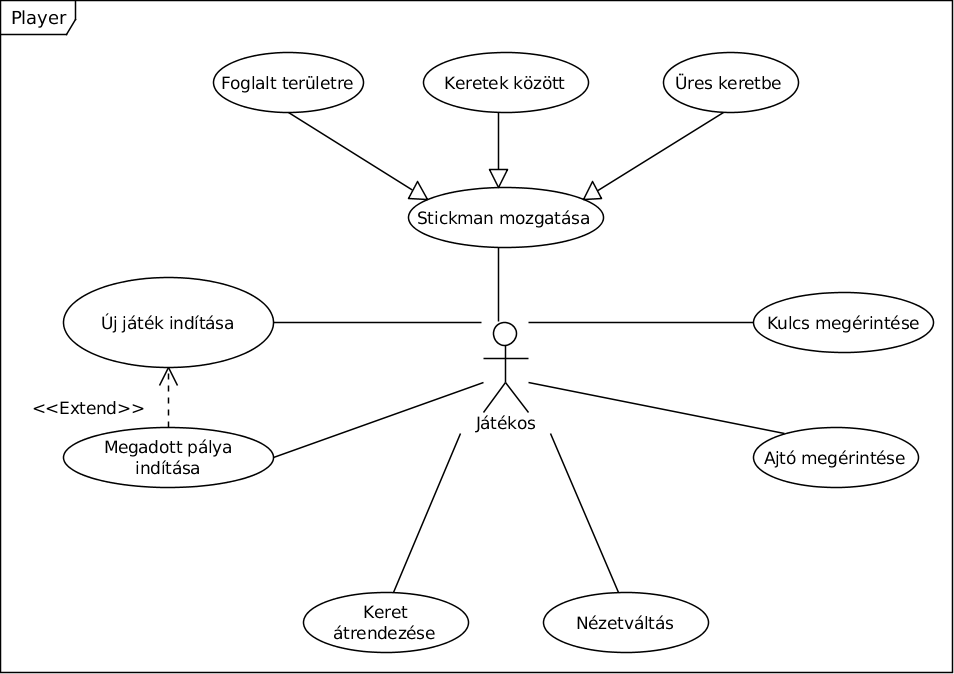
\includegraphics[scale=0.9]{resources/Player.png}
		    \end{center}
		
		\subsubsection{Játékos use case leírások}
		    Az alábbi use case leírások mindegyikének esetében az aktor a szkeleton programot kezelő Játékos.
		    
		    \begin{enumerate}[label=\textbf{\arabic*.}, start=1]
                \ucitem{Új játék indítása}
                    \ucdesc{A játékos új játékot indít.}
                    \ucscenario{Az új játék indítása során létrejön a játékot reprezentáló Game objektum, a pályákat előállító MapFactory, az időzítést végző Timer valamint az üzenetküldést segítő PubSub objektum. A Game objektum az inicializálás után betölti a MapFactory segítségével az első pályát.}
                    
                \ucitem{Megadott pálya indítása}
                    \ucdesc{A játékos meghatározza a betöltendő pályát.}
                    \ucscenario{Megegyezik az előzővel, azzal a különbséggel, hogy a Game objektum az első pálya helyett a megadott pályát tölti be.}
                    
                \ucitem{Stickman mozgatása}
                    \ucdesc{A játékos egy megadott irányba mozgatja a stickmant.}
                    \ucscenario{A Stickman objektum előállítja az elfoglalni kívánt Area objektumot, majd kérést intéz a tartalmazó Frame objektumhoz a terület elfoglalására. Amennyiben a terület szabad, az új területhez tartozó Frame beállítja a Stickman új helyét.}
                    
                \ucitem{(Stickman mozgatása) Foglalt területre.}
                    \ucdesc{A játékos olyan irányba szeretné mozgatni a stickmant, amerre Platform található.}
                    \ucscenario{Megegyezik az előzővel, azzal a különbséggel, hogy mivel az igényelt terület foglalt, a tartalmazó keret nem állít be új helyet, és false értékkel tér vissza}
                    
                \ucitem{(Stickman mozgatása) Keretek között}
                    \ucdesc{A játékos a stickmant a kerethatáron keresztül egy másik keretbe mozgatja.}
                    \ucscenario{A Stickman objektum előállítja az elfoglalni kívánt Area objektumot, majd kérést intéz a tartalmazó Frame objektumhoz a terület elfoglalására. Miután a tartalmazó keret meggyőződik arról, hogy a Stickman objektum elhagyja a területét, a Map objektumhoz fordul a szomszédjáért. A két keret közötti átjárhatóság és az új keretben elfoglalandó hely szabad mivolta ellenőrzésre kerül, a régi keret átadja a Stickman objektumot az új keretnek és az új keret állítja be az új pozíciót. Amennyiben az átjárhatóság vagy terület szabadsága nem teljesül, az eredeti keret false értékkel tér vissza, és nem állít be új pozíciót.}
                    
                \ucitem{(Stickman mozgatása) Üres keretbe}
                    \ucdesc{A játékos a stickmant a kerethatáron keresztül az üres keretbe mozgatja.}
                    \ucscenario{A Stickman objektum előállítja az elfoglalni kívánt Area objektumot, majd kérést intéz a tartalmazó Frame objektumhoz a terület elfoglalására. Miután a tartalmazó keret meggyőződik arról, hogy a Stickman objektum elhagyja a területét, a Map objektumhoz fordul a szomszédjáért. Mivel az adott irányban üres keret található, a Map objektum nullal tér vissza. Amennyiben a mozgás iránya lefelé mutat, a stickman kiesik és a keret visszaállítattja az utolsó ellenőrzőpontra. Más esetben false értékkel tér vissza, és nem állít be új pozíciót.}
                    
                \ucitem{Kulcs megérintése}
                    \ucdesc{A stickman mozgás során felvesz egy kulcsot.}
                    \ucscenario{Miután a stickman mozgatása miatt a tartalmazó keret beállította az új helyét, jelzi a kulcs objektumnak, hogy megérintették, amennyiben a stickman új helyének és a kulcs objektum által elfoglalt helynek van közös metszete.}
                    
                \ucitem{Ajtó megérintése}
                    \ucdesc{A stickman mozgás során egy ajtóhoz ér.}
                    \ucscenario{Miután a stickman mozgatása miatt a tartalmazó keret beállította az új helyét, jelzi az ajtó objektumnak, hogy megérintették, amennyiben a stickman új helyének és az ajtó objektum által elfoglalt helynek van közös metszete.}
                    
                \ucitem{Keret átrendezése}
                    \ucdesc{A játékos mozgat egy keretet.}
                    \ucscenario{A játékos megadja a mozgatás irányát. A Map objektum, mely a kereteket tartalmazza, megkeresi az üres keretet. Amennyiben a megadott iránnyal ellenkező irányban van szomszédja az üres keretnek, kicseréli a kettőt, ellenkező esetben tétlen. A keretek átrendezése nem igényel objektumok közötti kommunikációt, azt a Map objektum önmagában el tudja végezni.}
                    
                \ucitem{Nézetváltás}
                    \ucdesc{A játékos vált pálya és közeli nézet között.}
                    \ucscenario{Felhasználói interakció hatására a Game objektum állapota megváltozik, váltás történik pálya és közeli nézet között. Az állapotváltozás kommunikációt nem igényel, de befolyásolja a Timer actor egyes use case-eit.}
                    
		    \end{enumerate}
		    
		\subsubsection{Óra use case diagram}
		    \begin{center}
			    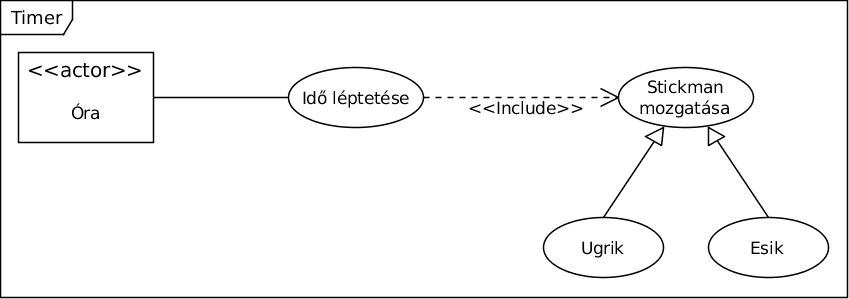
\includegraphics[scale=1]{resources/Timer.png}
		    \end{center}
		
		\subsubsection{Óra use case leírások}
		    Az alábbi use case leírások mindegyikének esetében az aktor az idő múlását követő óra (Timer).
		    
		    \begin{enumerate}[label=\textbf{\arabic*.}, start=1]
                \ucitem{Idő léptetése}
                    \ucdesc{A Timer objektum jelzi az idő múlását.}
                    \ucscenario{A Timer objektum előre meghatározott időközönként egy \texttt{tick} eseményt tesz közzé a megadott PubSub objektumon keresztül. Az időre érzékeny objektumok feliratkozhatnak erre az eseményre.}
                    
                \ucitem{Stickman mozgatása}
                    \ucdesc{Az idő múlásával a stickman közvetlen felhasználói interakció nélkül is mozoghat.}
                    \ucscenario{A Stickman objektum a \texttt{tick} esemény hatására -- mely az idő múlását jelzi -- felfelé mozoghat, amennyiben éppen ugrik, ellenkező esetben lefelé mozog (álló helyzetben is esik, mintha hatna rá a gravitációs gyorsulás).}
                    
                \ucitem{(Stickman mozgatása) Ugrik}
                    \ucdesc{Az idő múlásával a stickman egy folyamatos ugrást hajt végre.}
                    \ucscenario{A Stickman objektum a \texttt{tick} esemény hatására -- mely az idő múlását jelzi -- felfelé mozdul, vagyis ugrik. A felfelé történő mozgások száma egy előre meghatározott véges szám. A hátralévő ugrások száma minden egyes felfelé irányuló mozgással csökken.}
                    
                \ucitem{(Stickman mozgatása) Esik}
                    \ucdesc{Az idő múlásával a stickman folyamatosan esik.}
                    \ucscenario{A stickmanre minden pillanatban -- amikor nem ugrik -- lefele irányúló erő hat, ezért a \texttt{tick} esemény hatására -- amikor nincs alatta talaj -- lefelé mozdul (valójában folyamatosan lefelé mozdulna a talajon állva, de ezt a platform megakadályozza).}
		    \end{enumerate}
	
	\subsection{Architektúra}
		A szkeleton architektúrális felépítésének célja, hogy minden egyes use case tesztelhető legyen, valamint meg lehessen állapítani, hogy az előző -- analízisben rögzített -- szekvencia diagramoknak megfelelően működik-e az osztályok közötti kommunikáció. A tesztesetek futtatására előre inicializált pályák állnak majd rendelkezésünkre, hogy a fontos szituációk élesben is tesztelhetőek legyenek. A szkeleton tesztelése szekvenciálisan fog lefutni, ezért nincs szükség a konkurrens feladatok vizsgálatára.
		
		A tesztesetek úgy lettek megválasztva, hogy az adott használati eseteket legjobban mutassák be, minél kevesebb objektummal, hogy a vizsgálandó rész legyen a középpontban. A tesztesetek mellett feltüntettük az általuk használt frame-ek számát, a realizált objektumokat, illetve a tesztelés célját.
		
		Az alábbi tesztesetek az átláthatóság érdekében azon, az 5.1.2. és 5.1.4. use case leírásokban számozott használati esetek számát jelölik, amelyeket megvalósítanak (pl.: P1 -- 1. Játékos use case; T5 -- 5. Timer use case). A csillaggal jelölt use case-ek nagyon hasonlóak a teszteset által kijelölt fő use case-hez, ezért nem igényelnek külön tesztesetet.
								
		\begin{enumerate}[label=\textbf{\arabic*.}, start=0]
		
			\newcommand{\testitem}[1]{\item \textbf{Teszteset -- #1}\\}
			\newcommand{\tframe}[1]{\textbf{Frame-ek száma:} #1\\}
			\newcommand{\tobjekt}[1]{\textbf{Objektumok:} #1\\}
			\newcommand{\tcel}[1]{\textbf{Cél:} #1\\}
			\newcommand{\tuse}[1]{\textbf{Tesztelt use case:} #1\\}
		
			\testitem{Inicializálás}
				\tframe{1}
				\tobjekt{Minden, a futtatáshoz szükséges objektumtípusból legalább egy.
					(Game, Timer, PubSub, MapFactory, Map, Frame, Platform, Door, Key, Stickman stb.)}
				\tcel{Objektumok létrehozása, kapcsolatok kialakításának bemutatása.}
				\tuse{P1, *P2}
			\testitem{Stickman mozgatása}
				\tframe{1}
				\tobjekt{Frame, Stickman, Area, Timer}
				\tcel{A játékos mozdulni szeretne. Bemutatásra kerül a mozgás kérése és az arra kapott válasz, majd léptetés.} 
				\tuse{P3, *T2, *T1}
			\testitem{Stickman ugrása}
				\tframe{1}
				\tobjekt{Frame, Stickman, Timer}
				\tcel{A játékos ugrik, majd leesik, nincs akadály. Idő által kiváltott metódushívások figyelhetőek meg.} 
				\tuse{T3, *T1}
			\testitem{Stickman mozgatása foglalt területre}
				\tframe{1}
				\tobjekt{Frame, Stickman, Platform, Area}
				\tcel{A játékos mozdulni szeretne, de platform állja el az útját. Előzőhöz hasonlóan bemutatható a kommunikáció, kivéve hogy a mozgás kérésre nem kap engedélyt, pozíciója nem fog változni.}
				\tuse{P4}
			\testitem{Stickman mozgatása keretek között}
				\tframe{2}
				\tobjekt{Map, 2 db. Frame, Stickman, Area}
				\tcel{Játékos mozdulni szeretne a jelenlegi keretet elhagyva. Az előzőekhez hasonlóan a kommunikáció bemutatható a Stickman -- Frame, illetve itt a Frame -- Map objektumok között.}
				\tuse{P5}
			\testitem{Stickman mozgatása üres keretbe horizontálisan}
				\tframe{2}
				\tobjekt{Map, 2 db. Frame, Stickman, Area}
				\tcel{Stickman -- Frame, Frame -- Map kommunikáció bemutatása, lépés megtagadásával (nincs Frame).}
				\tuse{P6}
			\testitem{Stickman kiesése keretből}
				\tframe{2}
				\tobjekt{Map, 2 db. Frame, Stickman, Area, Timer}
				\tcel{Stickman -- Frame, Frame -- Map kommunikáció bemutatása, utolsó ellenőrzőpontra visszaállítás.}
				\tuse{P6, *T4, *T1}
			\testitem{Kulcs felvétele}
				\tframe{1}
				\tobjekt{PubSub, Frame, Stickman, Key, Area}
				\tcel{A játékos kulcsot tartalmazó mezőbe lép, kulcs felvétele. Üzenet terjedésének bemutatása.}
				\tuse{P7}
			\testitem{Ajtó megérintése}
				\tframe{1}
				\tobjekt{PubSub, Frame, Stickman, Door, Area}
				\tcel{A játékos az ajtót tartalmazó mezőbe lép. Üzenet terjedésének bemutatása.}
				\tuse{P8}
			\testitem{Keret átrendezése}
				\tframe{2}
				\tobjekt{Map, 2 db. Frame}
				\tcel{A játékos keretet próbál mozgatni. Objektumok nem kommunikálnak, a Map magában intézi a mozgást, ha a mozgatás irányával ellentétes irányban van keret az üres keret mellett.}
				\tuse{P9}
			\testitem{Nézetváltás}
				\tframe{1}
				\tobjekt{Game}
				\tcel{A játékos a megfelelő gomb megnyomásával nézetet vált. A Game objektumban lesz állapotváltozás, kommunikáció nem szükséges.}
				\tuse{P10}
		\end{enumerate}
	
	\subsection{A szkeleton kezelői felületének terve, dialógusok}
		A szkeleton, mint program célja annak bizonyítása, hogy a programunk statikus és dinamikus modelljeiről leképzett programváz képes az elvárt működést produkálni. A szkeletonban minden objektum szerepel, de azoknak csak az interfésze definiált.
		
		A szkeleton működését össze kell tudnunk vetni az elkészített szekvencia diagramokkal. Ezt úgy érjük el, hogy minden egyes metódushíváskor kiírjuk a konzolra a hívott metódus és osztály nevét, az objektum azonosítóját, valamint az átadott paraméterek jellemzőit. A metódusból való visszatérésnél ezt újra megtesszük, és kiegészítjük a visszatérési értékkel. Jelen esetben az objektum azonosítását a Java beépített hash code attribútumának segítségével fogjuk megoldani. A könnyebb eligazodás kedvéért a metódushívási hierarchiának megfelelő behúzást használunk.
		
		Mivel a szkeletonból hiányzik az üzleti logika megvalósítása, ezért a feltételes elágazásoknál felhasználói interakcióra van szükség. Ilyenkor megállítjuk a programot, a konzolon egy kérdést jelenítünk meg, majd miután a felhasználó bevitte a megfelelő értéket, folytatjuk a program futását.
		
		\subsubsection*{Metódushívás során megjelenített adatok}
			\begin{itemize}
				\item Osztály neve
				\item Objektum azonosítója (hash code)
				\item Metódus neve
				\item Paraméterlista: osztálynév, objektumazonosító
			\end{itemize}					
		
		\subsubsection*{Minta kimenet}
			\begin{verbatim}
			-> Map[867].addItem(FrameItem[868])
			  -> FrameItem[868].getArea()
			  <- FrameItem[868].getArea() :: Area[869]
			  < Is frame at area? (y/n)
			  > y
			  -> Frame[450].addItem(FrameItem[868])
			    -> FrameItem[868].setFrame(Frame[450])
			    <- FrameItem[868].setFrame(Frame[450])
			  <- Frame[450].addItem(FrameItem[868])
			  -> Area[870].Area()
			  <- Area[870].Area()
			  -> FrameItem[868].setArea(Area[870])
			  <- FrameItem[868].setArea(Area[870])
			<- Map[867].addItem(FrameItem[868])
			\end{verbatim}
	
	\subsection{Szekvencia diagramok a belső működésre}
	
		\begin{center}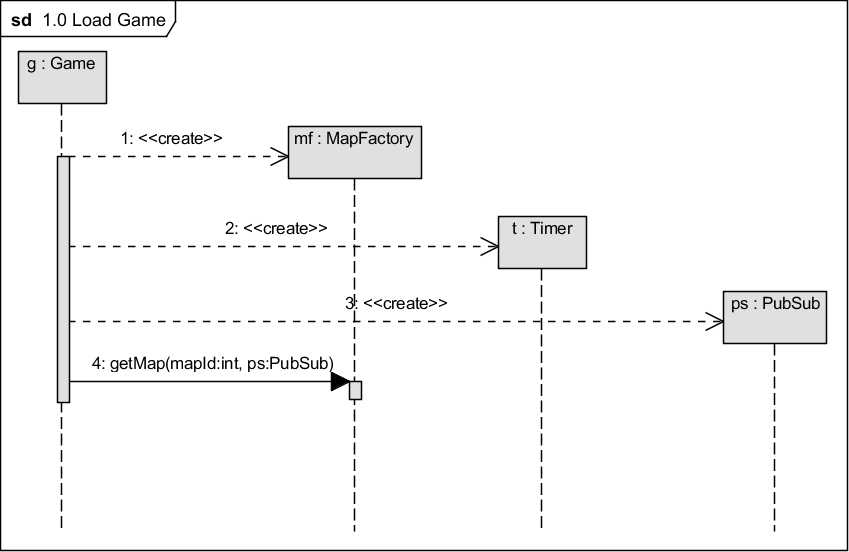
\includegraphics[scale=1]{resources/10LoadGame.png}\end{center}
		\begin{center}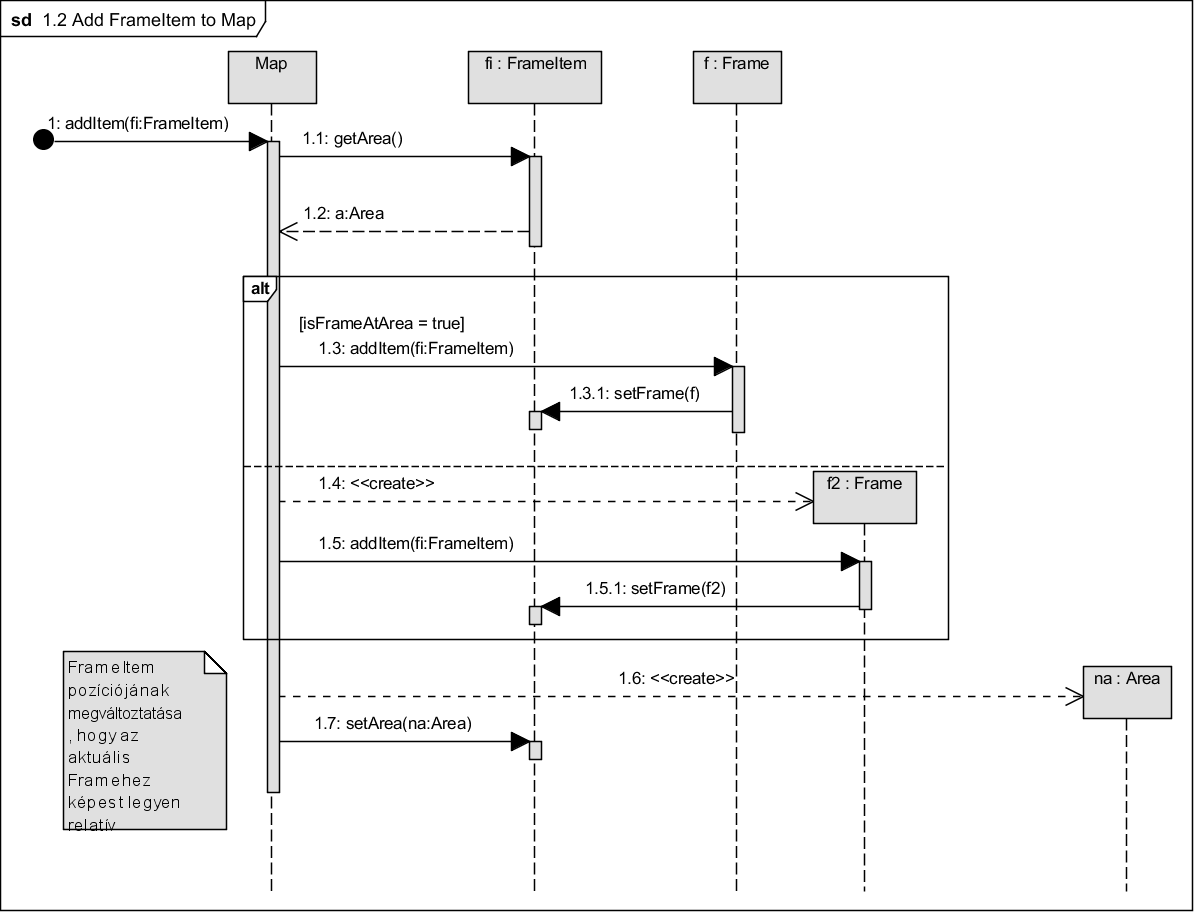
\includegraphics[scale=0.75]{resources/12AddFrameItemtoMap.png}\end{center}
		\begin{center}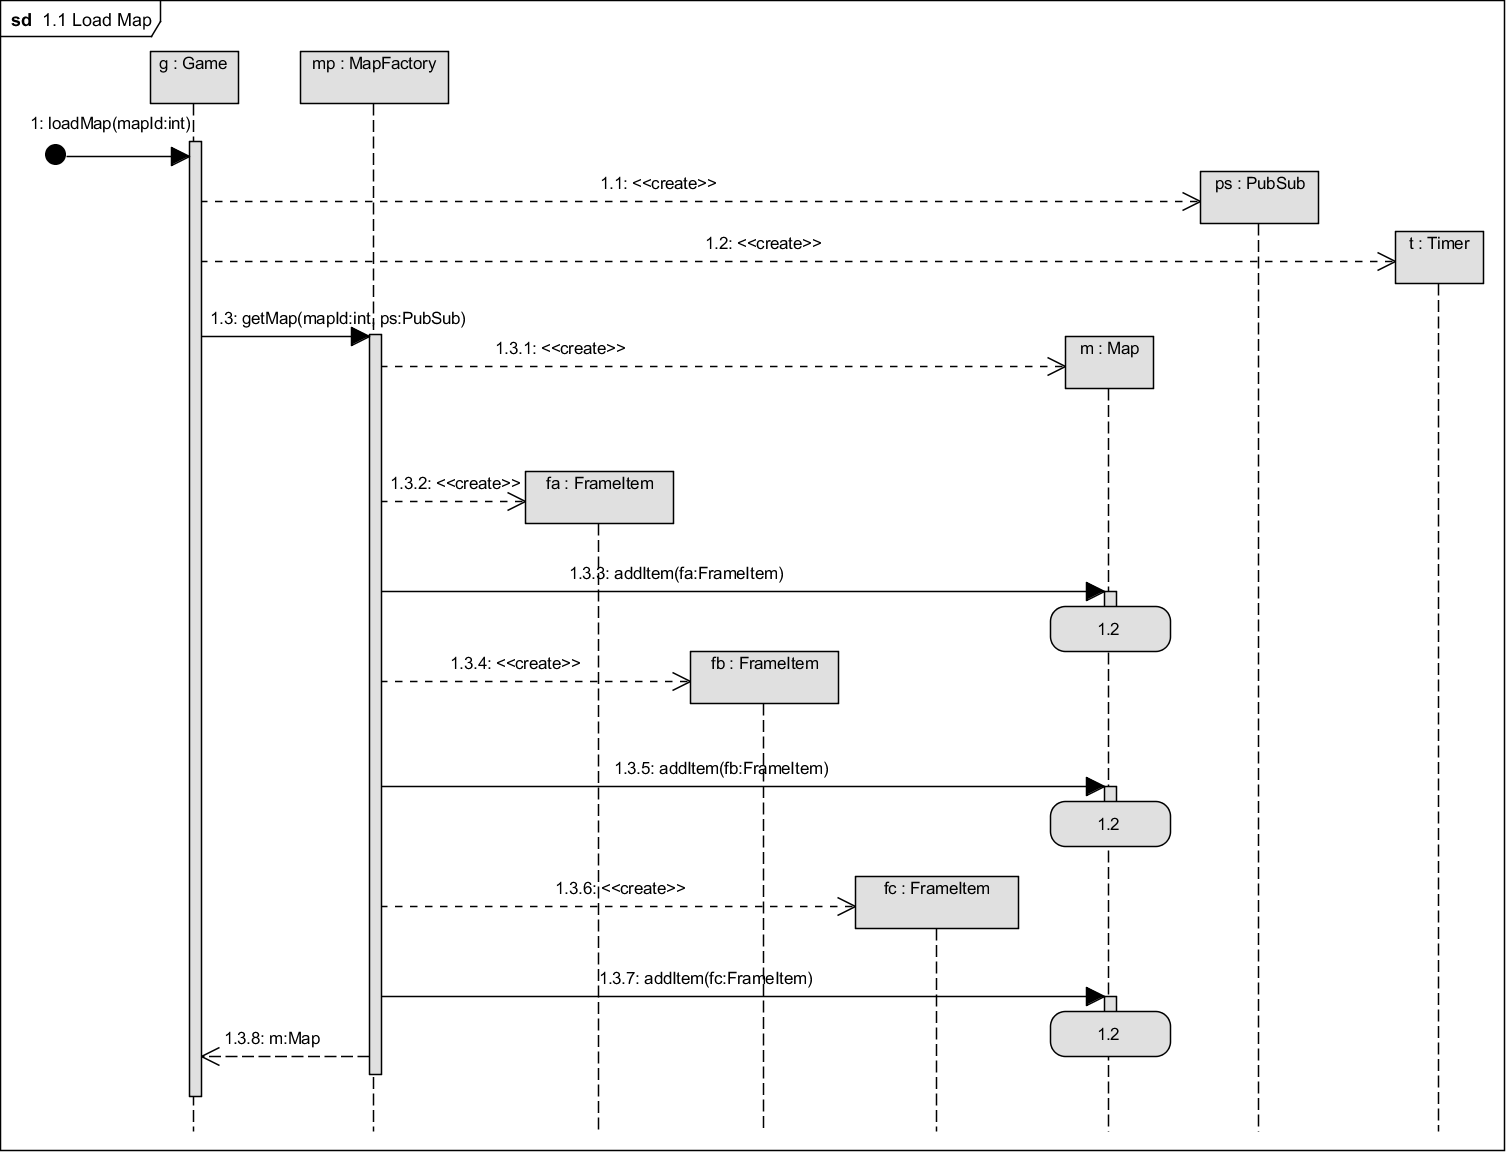
\includegraphics[scale=0.8, angle=-90]{resources/11LoadMap.png}\end{center}
		\begin{center}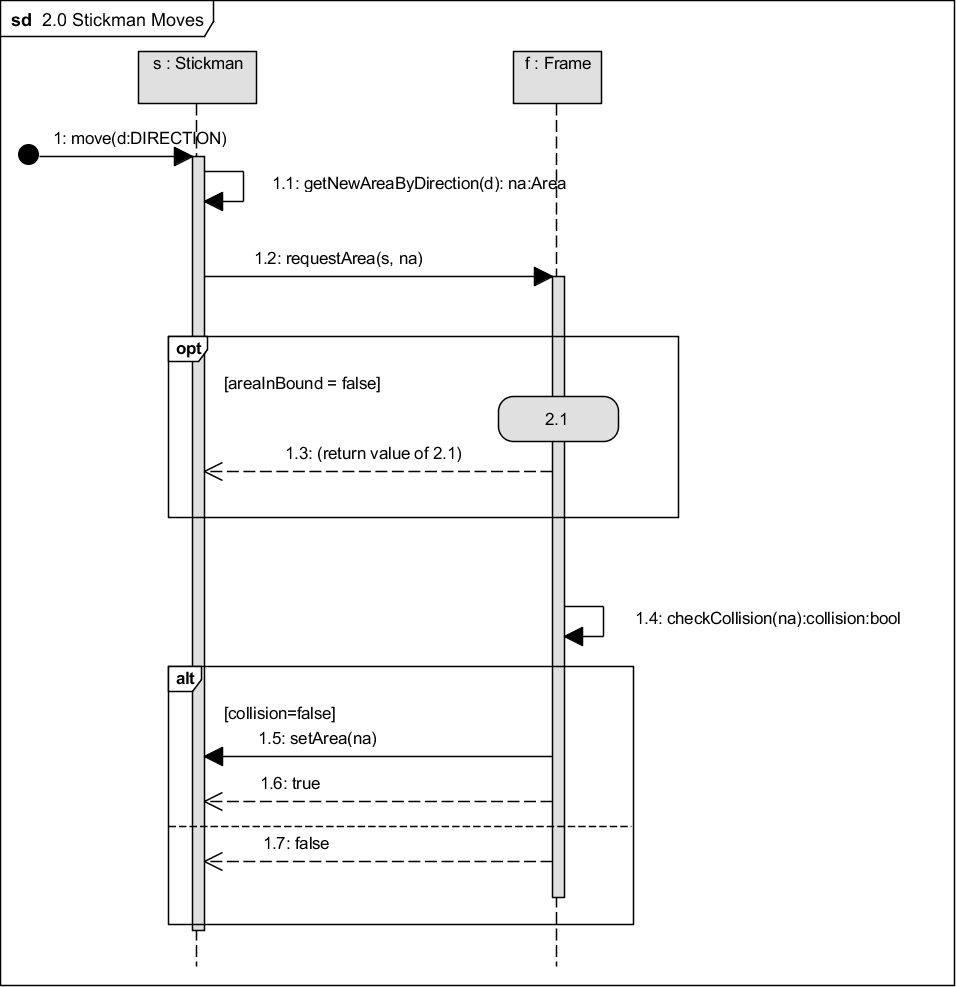
\includegraphics[scale=0.95]{resources/20StickmanMoves.png}\end{center}
		\begin{center}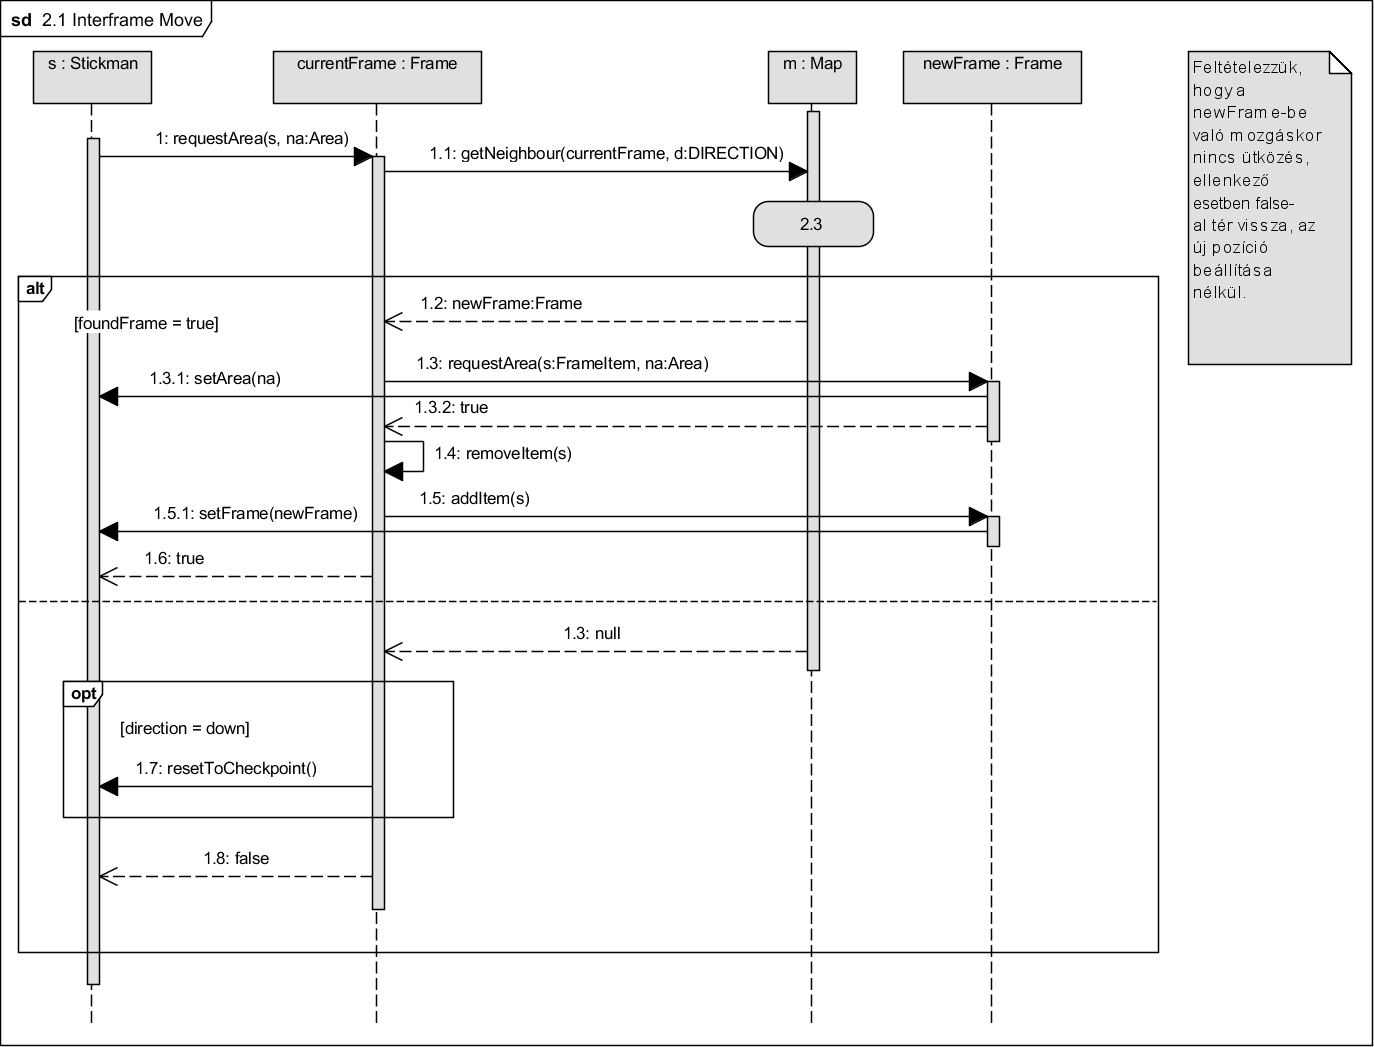
\includegraphics[scale=0.8, angle=-90]{resources/21InterframeMove.png}\end{center}
		\begin{center}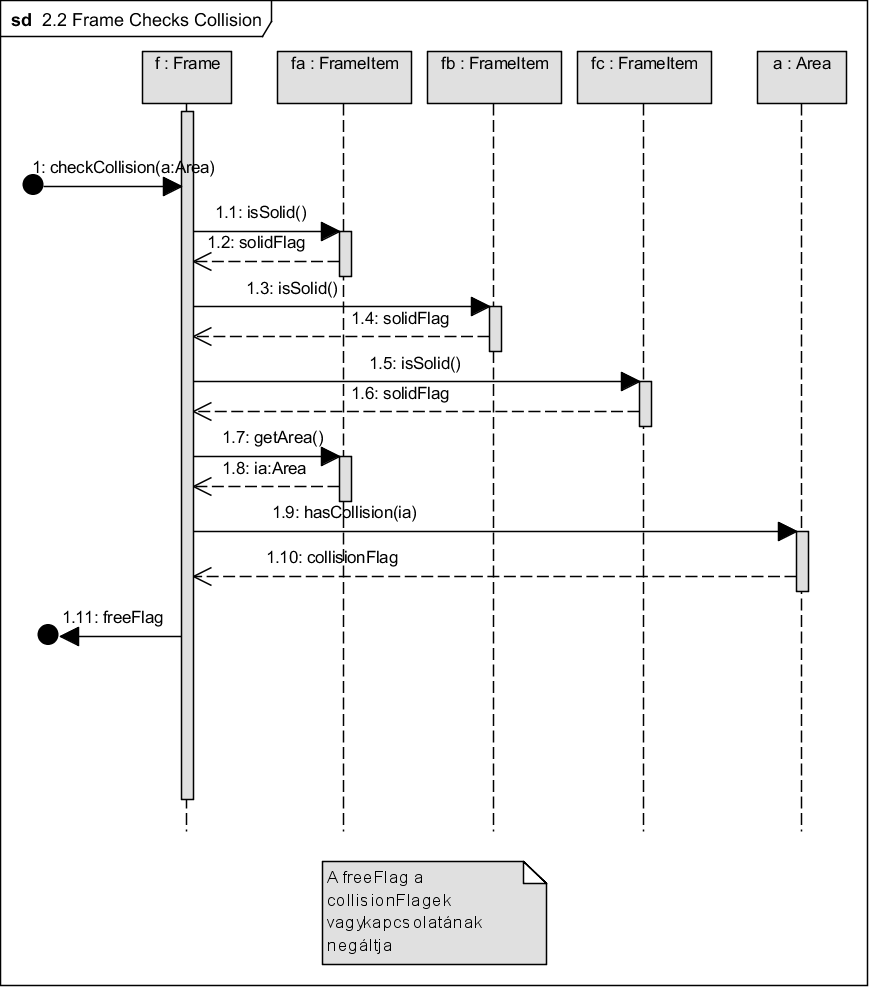
\includegraphics[scale=1]{resources/22FrameChecksCollision.png}\end{center}
		\begin{center}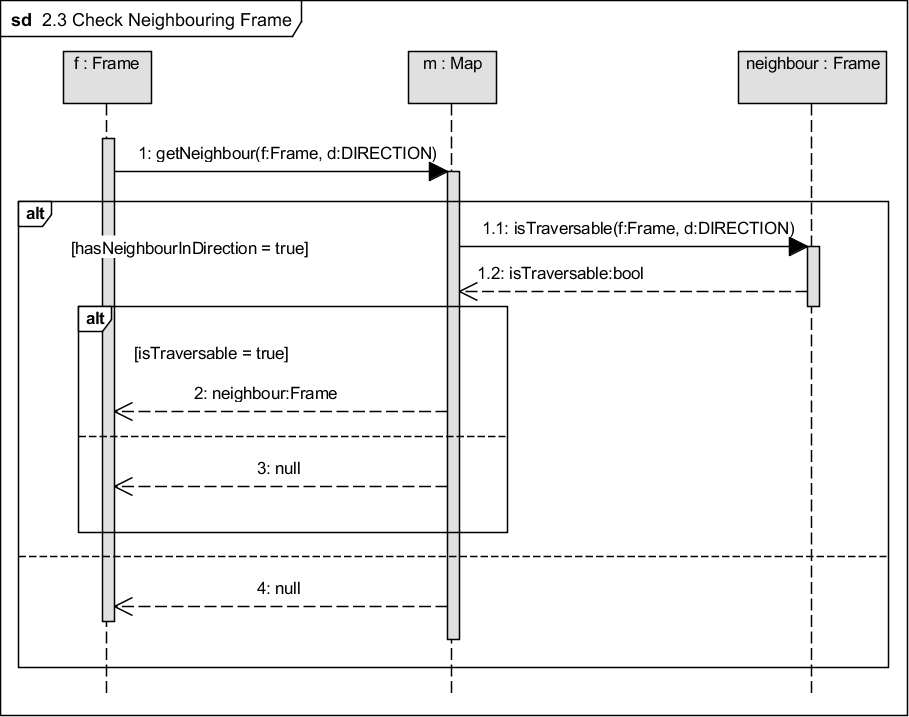
\includegraphics[scale=1]{resources/23CheckNeighbouringFrame.png}\end{center}
		\begin{center}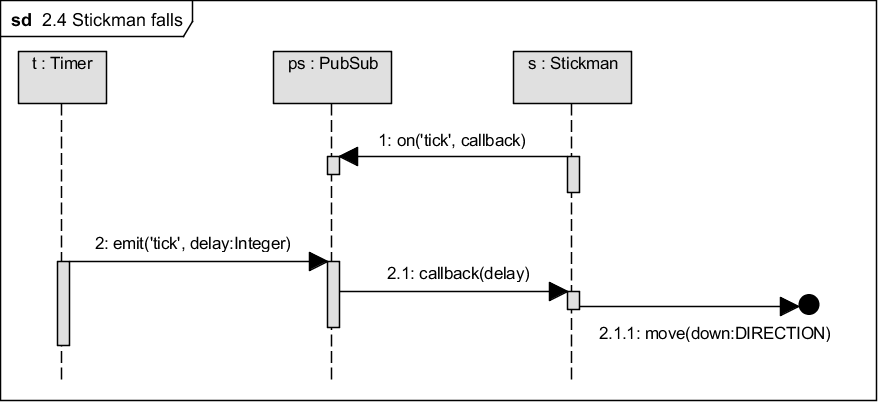
\includegraphics[scale=1]{resources/24Stickmanfalls.png}\end{center}
		\begin{center}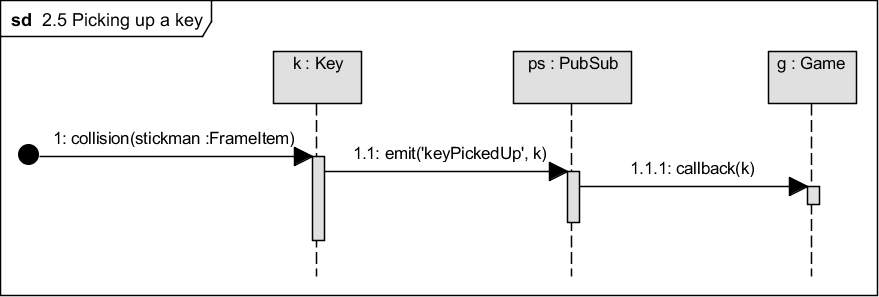
\includegraphics[scale=1]{resources/25Pickingupakey.png}\end{center}
		\begin{center}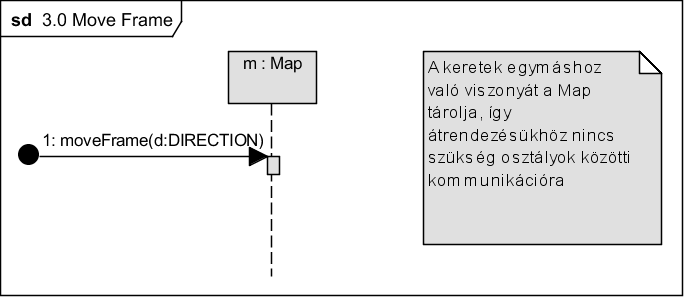
\includegraphics[scale=1]{resources/30MoveFrame.png}\end{center}
		\begin{center}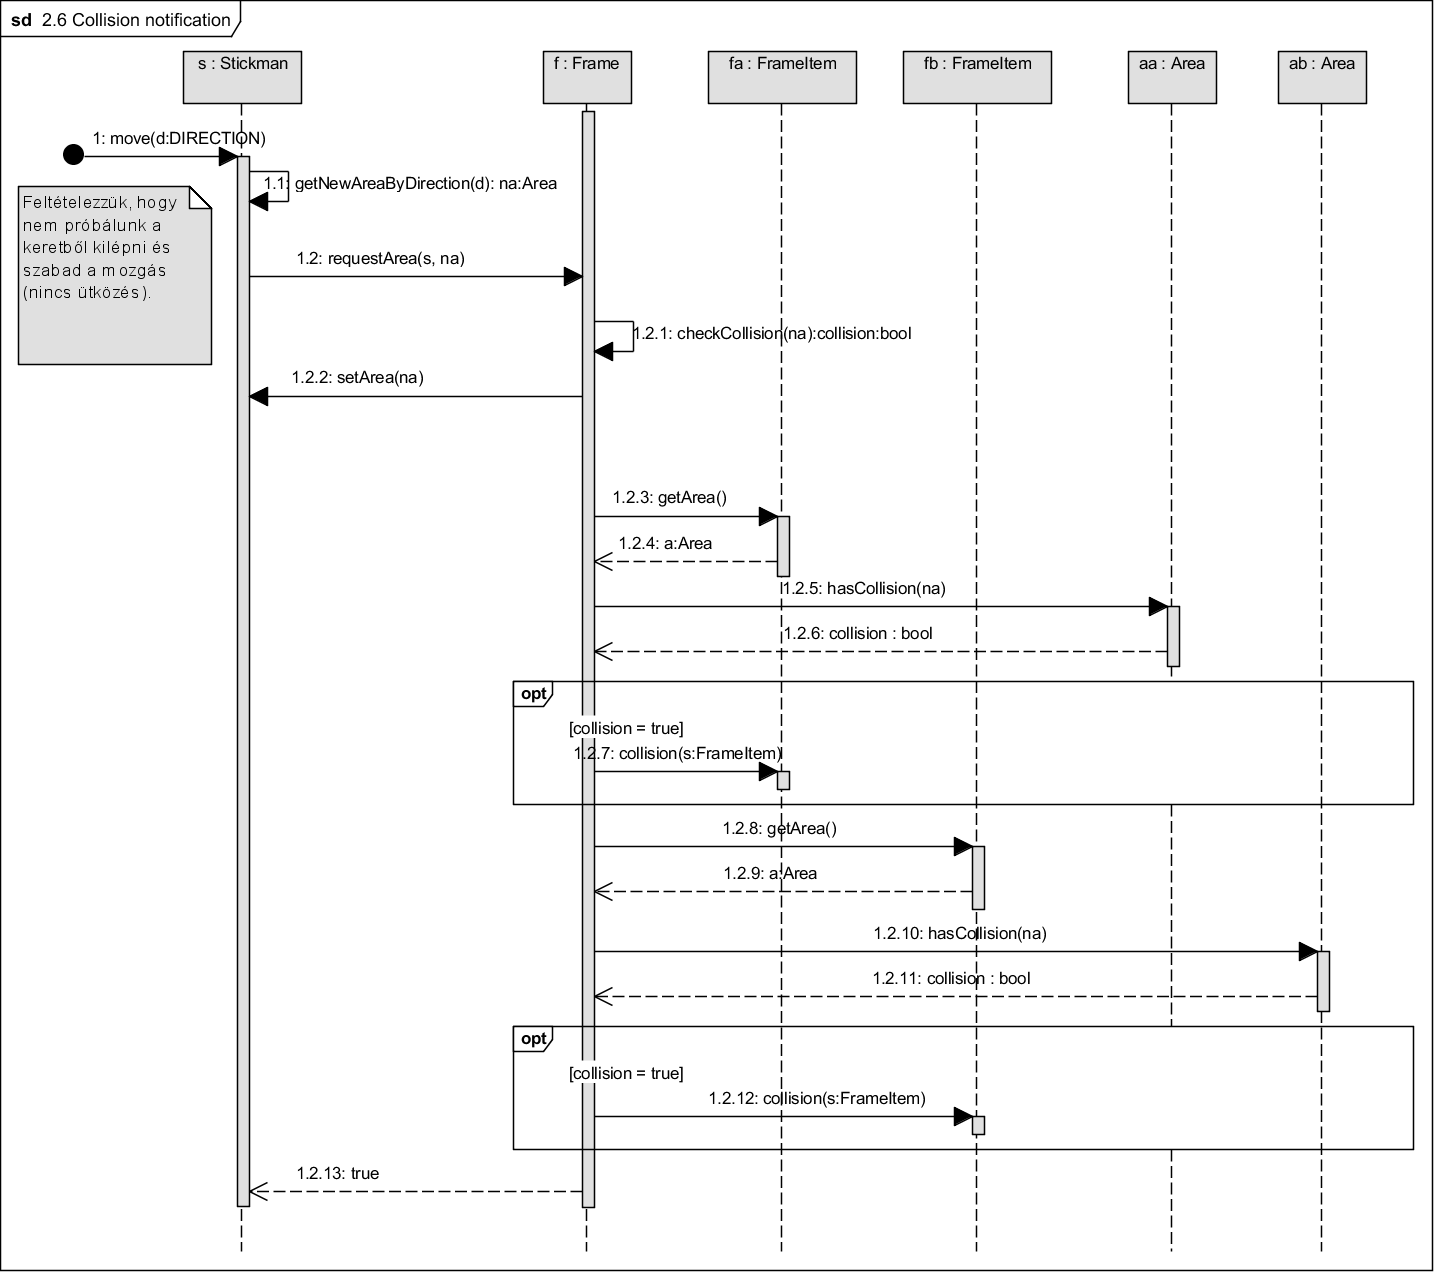
\includegraphics[scale=0.7, angle=-90]{resources/26Collisionnotification.png}\end{center}
	
	\subsection{Napló}
	% The diary generator uses the following comments to identify the beginning and the ending of the generated diary
	% The following content is auto generated, please do NOT modify, edit the related shared document instead.
	%GENERATOR:DIARY
    \begin{center} 
        \begin{tabular}{| l | p{1.9cm} | p{2.6cm} | p{6.1cm} |}
            \hline
                Kezdet & Időtartam & Résztvevők & Leírás \\
            \hline \hline 
2012. 03. 09. 17:00 & 3 óra & Berki & Szekvencia diagramok\\ \hline
2012. 03. 10. 18:00 & 2 óra & Fodor & A szkeleton kezelői felület tervének kidolgozása\\ \hline
2012. 03. 10. 21:20 & 2 óra & Kádár & Architektúra\\ \hline
2012. 03. 11. 11:30 & 2 óra & Thaler & Use case diagram\\ \hline
2012. 03. 11. 14:30 & 1 óra & Thaler & Use case diagram\\ \hline
2012. 03. 11. 15:30 & 1.5 óra & Kádár & Architektúra\\ \hline
2012. 03. 11. 22:00 & 1.5 óra & Thaler & Javítások, Napló, zárás\\ \hline
2012. 03. 11. 22:00 & 1.5 óra & Fodor & Javítások\\ \hline
2012. 03. 12. 08:30 & 0.5 óra & Kádár & Nyomtatás, átnézés\\ \hline

            \hline
        \end{tabular}
    \end{center}
	%GENERATOR:DIARY
\end{document}
